\documentclass[11pt,letterpaper]{article}
\usepackage[utf8]{inputenc}
\usepackage[left=.5in,right=.5in,top=.5in,bottom=.5in]{geometry} 

%\usepackage[margin=.5in]{geometry} % see geometry.pdf on how to lay out the page. There's lots.
%\geometry{a4paper} % or letter or a5paper or ... etc
%\usepackage{fullpage}
\usepackage{amsfonts}
%\usepackage[margin=0.5in]{geometry}
% \geometry{landscape} % rotated page geometry
%\addtolength{\oddsidemargin}{-.875in}
%\addtolength{\evensidemargin}{-.875in}
%\addtolength{\textwidth}{1.75in}
%
%\addtolength{\topmargin}{-1.375in}
%\addtolength{\textheight}{1.875in}
\usepackage{framed}
\usepackage{makebox}
\usepackage{minibox}
\usepackage{graphicx}
\usepackage{caption}
%\usepackage{fullpage}
\usepackage{graphicx}
\usepackage{caption}
\usepackage{subcaption}
\usepackage{xcolor}
% \usepackage{mdframed}
\usepackage{lipsum}
\usepackage{textcomp}
\usepackage{wrapfig}
\usepackage{setspace}
\usepackage{amsmath}
\usepackage{breqn}
\usepackage{amsmath}
\usepackage{amsfonts}
\usepackage{amssymb}
\usepackage{setspace}
\usepackage{hyperref}

% LaTeXML-friendly environments
\newenvironment{solution}{\par\medskip\noindent\textbf{Solution.}\par}{\medskip}
\newenvironment{keyidea}{\par\medskip\noindent\textbf{Key Idea.}\par}{\medskip}

\usepackage{textcomp} 
\usepackage{multicol} 
 
\newcounter{NumberInTable}
\newcommand{\LTNUM}{\stepcounter{NumberInTable}{(\theNumberInTable)}}

\newcommand{\Laplace}[1]{\ensuremath{\mathcal{L}{\left[#1\right]}}}
\newcommand{\InvLap}[1]{\ensuremath{\mathcal{L}^{-1}{\left[#1\right]}}}
\DeclareMathOperator{\arcsec}{arcsec}
\DeclareMathOperator{\arccot}{arccot}
\DeclareMathOperator{\arccsc}{arccsc}

\colorlet{shadecolor}{blue!15}

\newtheorem{theorem}{Theorem}

\newenvironment{theo}
  {\begin{shaded}\begin{theorem}}
  {\end{theorem}\end{shaded}}

\usepackage{numprint}

%%% BEGIN DOCUMENT
\begin{document}
\begin{center}
\Large Math 252, 10.3, Calculus of Parametric Equations\normalsize\vspace{.1in}\\
\end{center}
\begin{enumerate}
\item \textbf{Motivation.} Consider again, a ball is thrown so that it's path $x=24\sqrt{2}t$ and $y=-16t^{2}+24\sqrt{2}t$, where $t$ is time in seconds.  How could we determine it's velocity and acceleration?

The horizontal and vertical components of velocity are
\[
\frac{dx}{dt}=24\sqrt{2}
\qquad\text{and}\qquad
\frac{dy}{dt}=-32t+24\sqrt{2}.
\]
Thus, the velocity vector is
\[
\mathbf{v}(t)=\left\langle 24\sqrt{2},-32t+24\sqrt{2}\right\rangle.
\]
The horizontal and vertical components of acceleration are
\[
\frac{d^{2}x}{dt^{2}}=0
\qquad\text{and}\qquad
\frac{d^{2}y}{dt^{2}}=-32.
\]
Thus, the acceleration vector is
\[
\mathbf{a}(t)=\langle 0,-32\rangle.
\]

\item \textbf{Derivation of Derivative Formulas} \\
\begin{center}
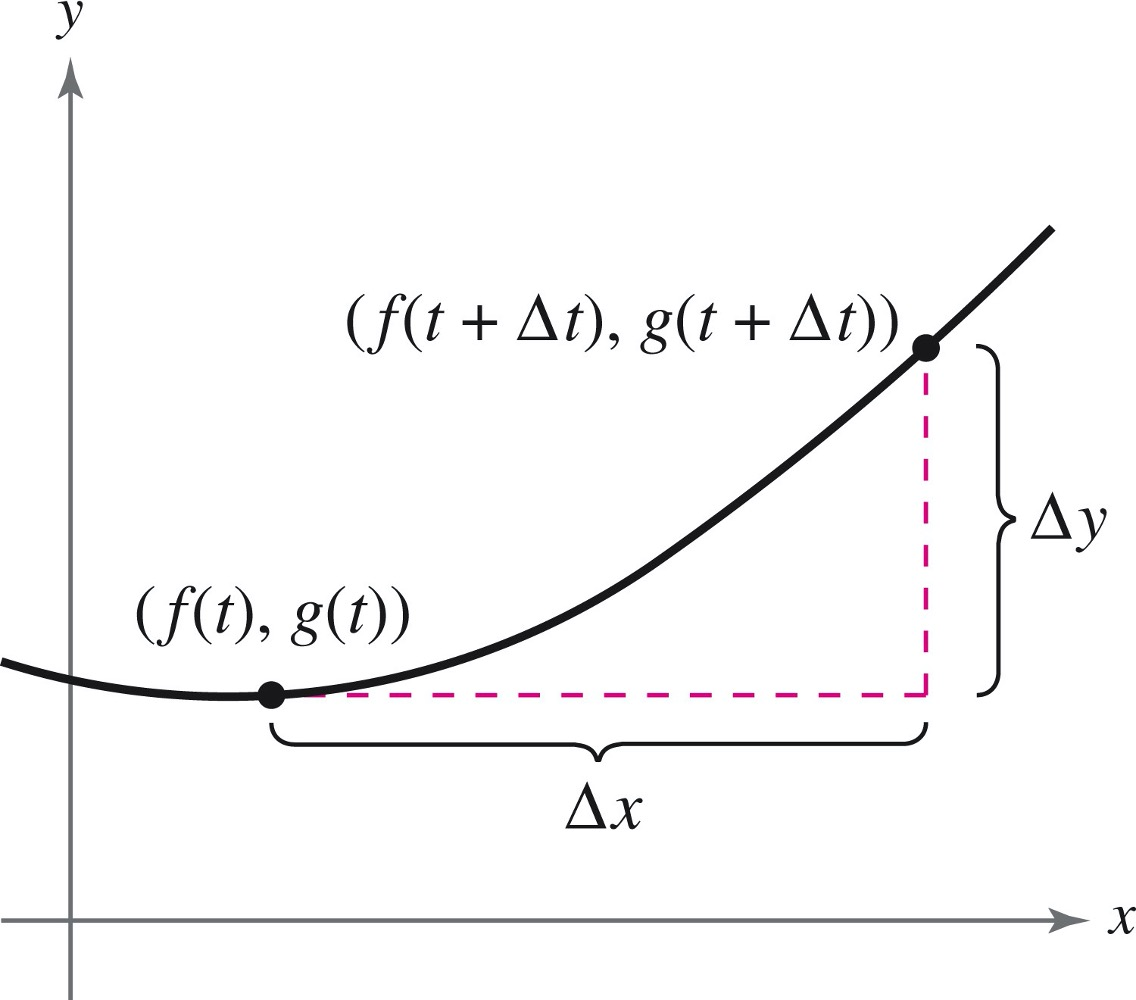
\includegraphics[scale=.2]{Picture1.jpg}
\end{center}

Suppose that a parametric curve is given by
\[
x=f(t)
\qquad\text{and}\qquad
y=g(t).
\]
Consider the points on the curve corresponding to the parameter values $t$ and
$t+\Delta t$:
\[
P=\bigl(f(t),g(t)\bigr)
\qquad\text{and}\qquad
Q=\bigl(f(t+\Delta t),g(t+\Delta t)\bigr).
\]
The slope of the secant line through $P$ and $Q$ is
\begin{eqnarray*}
\frac{\Delta y}{\Delta x}
&=&
\frac{g(t+\Delta t)-g(t)}
     {f(t+\Delta t)-f(t)}\\
&=&
\frac{\dfrac{g(t+\Delta t)-g(t)}{\Delta t}}
     {\dfrac{f(t+\Delta t)-f(t)}{\Delta t}}.
\end{eqnarray*}
As $\Delta t\longrightarrow 0$, the point $Q$ approaches the point $P$, and
the secant line approaches the tangent line.  Therefore,
\begin{eqnarray*}
\frac{dy}{dx}
&=&
\lim_{\Delta t\to0}
\frac{\dfrac{g(t+\Delta t)-g(t)}{\Delta t}}
     {\dfrac{f(t+\Delta t)-f(t)}{\Delta t}}\\
&=&
\frac{\displaystyle\lim_{\Delta t\to0}
\dfrac{g(t+\Delta t)-g(t)}{\Delta t}}
{\displaystyle\lim_{\Delta t\to0}
\dfrac{f(t+\Delta t)-f(t)}{\Delta t}}\\
&=&
\frac{g'(t)}{f'(t)}\\
&=&
\frac{dy/dt}{dx/dt},
\end{eqnarray*}
provided $\dfrac{dx}{dt}\neq0$.

% \newpage
\item \textbf{Example 1:} Let $x=\sin t$ and $y=\cos t$.  Find $dy/dx$

\[
\frac{dx}{dt}=\cos t
\qquad\text{and}\qquad
\frac{dy}{dt}=-\sin t.
\]
Therefore,
\[
\frac{dy}{dx}
=
\frac{dy/dt}{dx/dt}
=
\frac{-\sin t}{\cos t}
=
-\tan t.
\]\\
\item \textbf{Higher Order Derivatives.}

We know that
\[
\frac{dy}{dx}=\frac{dy/dt}{dx/dt}.
\]
To find the second derivative, differentiate the first derivative with
respect to $x$:
\[
\frac{d^{2}y}{dx^{2}}
=
\frac{d}{dx}\left(\frac{dy}{dx}\right).
\]
Using the first derivative formula with
\[
y=\frac{dy}{dx},
\]
we obtain
\[
\frac{d^{2}y}{dx^{2}}
=
\frac{\dfrac{d}{dt}\left(\dfrac{dy}{dx}\right)}
     {\dfrac{dx}{dt}}.
\]
Since
\[
\frac{dy}{dx}=\frac{dy/dt}{dx/dt},
\]
it follows that
\[
\boxed{
\frac{d^{2}y}{dx^{2}}
=
\frac{\dfrac{d}{dt}\left(\dfrac{dy/dt}{dx/dt}\right)}
     {\dfrac{dx}{dt}}
}.
\]
\item \textbf{Example 2:} For the curve $x=\sqrt{t}$ and $\displaystyle y=\frac{1}{4}(t^{2}-4)$, for $t\geq0$, find the slope and concavity at the point $(2,3)$.

At the point $(2,3)$,
\[
2=\sqrt{t},
\]
so
\[
t=4.
\]
Now,
\[
\frac{dx}{dt}=\frac{1}{2\sqrt{t}}
\qquad\text{and}\qquad
\frac{dy}{dt}=\frac{t}{2}.
\]
Thus,
\begin{eqnarray*}
\frac{dy}{dx}
&=&
\frac{dy/dt}{dx/dt}\\
&=&
\frac{t/2}{1/(2\sqrt{t})}\\
&=&
t\sqrt{t}.
\end{eqnarray*}
At $t=4$,
\[
\frac{dy}{dx}=4\sqrt{4}=8.
\]
Therefore, the slope at $(2,3)$ is $8$.

For concavity,
\begin{eqnarray*}
\frac{d^{2}y}{dx^{2}}
&=&
\frac{\dfrac{d}{dt}\left(\dfrac{dy}{dx}\right)}
     {\dfrac{dx}{dt}}\\
&=&
\frac{\dfrac{d}{dt}\left(t^{3/2}\right)}
     {1/(2\sqrt{t})}\\
&=&
\frac{\dfrac{3}{2}\sqrt{t}}
     {1/(2\sqrt{t})}\\
&=&
3t.
\end{eqnarray*}
At $t=4$,
\[
\frac{d^{2}y}{dx^{2}}=12>0.
\]
Therefore, the curve is concave upward at $(2,3)$.

% \newpage
\item \textbf{Example 3:}  The prolate cycloid is given by, $x=2t-\pi\sin t$ and $y=2-\pi \cos t$.  The curve crosses itself at the point $(0,2)$, as shown.  Find the equation of the tangent lines at this point.
\begin{center}
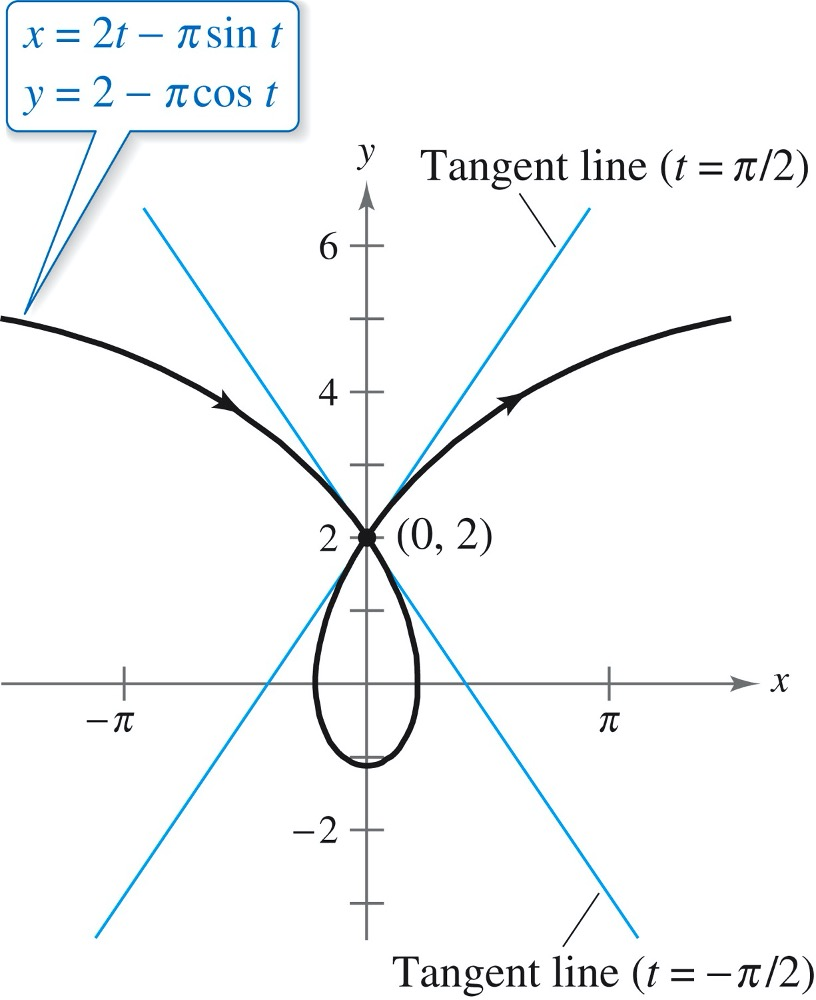
\includegraphics[scale=.2]{Picture4.jpg}
\end{center}

At the point $(0,2)$,
\[
2-\pi\cos t=2,
\]
so
\[
\cos t=0.
\]
The two parameter values at which the curve passes through $(0,2)$ are
\[
t=\frac{\pi}{2}
\qquad\text{and}\qquad
t=-\frac{\pi}{2}.
\]
Indeed,
\[
2\left(\frac{\pi}{2}\right)-\pi\sin\left(\frac{\pi}{2}\right)=0
\]
and
\[
2\left(-\frac{\pi}{2}\right)-\pi\sin\left(-\frac{\pi}{2}\right)=0.
\]

Now,
\[
\frac{dx}{dt}=2-\pi\cos t
\qquad\text{and}\qquad
\frac{dy}{dt}=\pi\sin t.
\]
Thus,
\[
\frac{dy}{dx}
=
\frac{\pi\sin t}{2-\pi\cos t}.
\]
At $t=\dfrac{\pi}{2}$,
\[
\frac{dy}{dx}=\frac{\pi}{2}.
\]
Therefore, one tangent line is
\[
y-2=\frac{\pi}{2}x.
\]
At $t=-\dfrac{\pi}{2}$,
\[
\frac{dy}{dx}=-\frac{\pi}{2}.
\]
Therefore, the other tangent line is
\[
y-2=-\frac{\pi}{2}x.
\]
\item \textbf{Arc Length} Consider a curve $C$ whose equation is given by $y=h(x)$.  If we want to find the length of the arc between $x_{0}$ and $x_{1}$, recall we have the formiula
\begin{eqnarray*}
s &=& \int_{x_{0}}^{x_{1}} \sqrt{1+[h'(x)]^{2}}\, dx\\
&=& \int_{x_{0}}^{x_{1}} \sqrt{1+[dy/dx]^{2}}\, dx\\
\end{eqnarray*}
Suppose that $x=f(t)$ and $y=g(t)$, where $t_{0}\leq t\leq t_{1}$.
Since
\[
\frac{dy}{dx}=\frac{dy/dt}{dx/dt}
\qquad\text{and}\qquad
dx=\frac{dx}{dt}\,dt,
\]
we have
\begin{eqnarray*}
s
&=&
\int_{t_{0}}^{t_{1}}
\sqrt{1+\left[\dfrac{dy/dt}{dx/dt}\right]^{2}}\,
\frac{dx}{dt}\,dt\\
&=&
\int_{t_{0}}^{t_{1}}
\sqrt{
\frac{(dx/dt)^{2}+(dy/dt)^{2}}
     {(dx/dt)^{2}}
}\,
\frac{dx}{dt}\,dt\\
&=&
\int_{t_{0}}^{t_{1}}
\sqrt{
\left(\frac{dx}{dt}\right)^{2}
+
\left(\frac{dy}{dt}\right)^{2}
}\,dt.
\end{eqnarray*}
Therefore, the arc length of a parametric curve is
\[
\boxed{
s=
\int_{t_{0}}^{t_{1}}
\sqrt{
\left(\frac{dx}{dt}\right)^{2}
+
\left(\frac{dy}{dt}\right)^{2}
}\,dt
}.
\]

% \newpage
\item \textbf{Example 4:} A circle of radius 1 rolls around the circumference of a large circle of radius 4.  If a point on the smaller circle is traced, the result is called an epicycloid, and its equation is given parametrically by $x=5\cos t-\cos 5t$ and $y=5\sin t-\sin 5t$.   Determine the distance traveled by the point in one complete trip around the larger circle.\\
\begin{center}
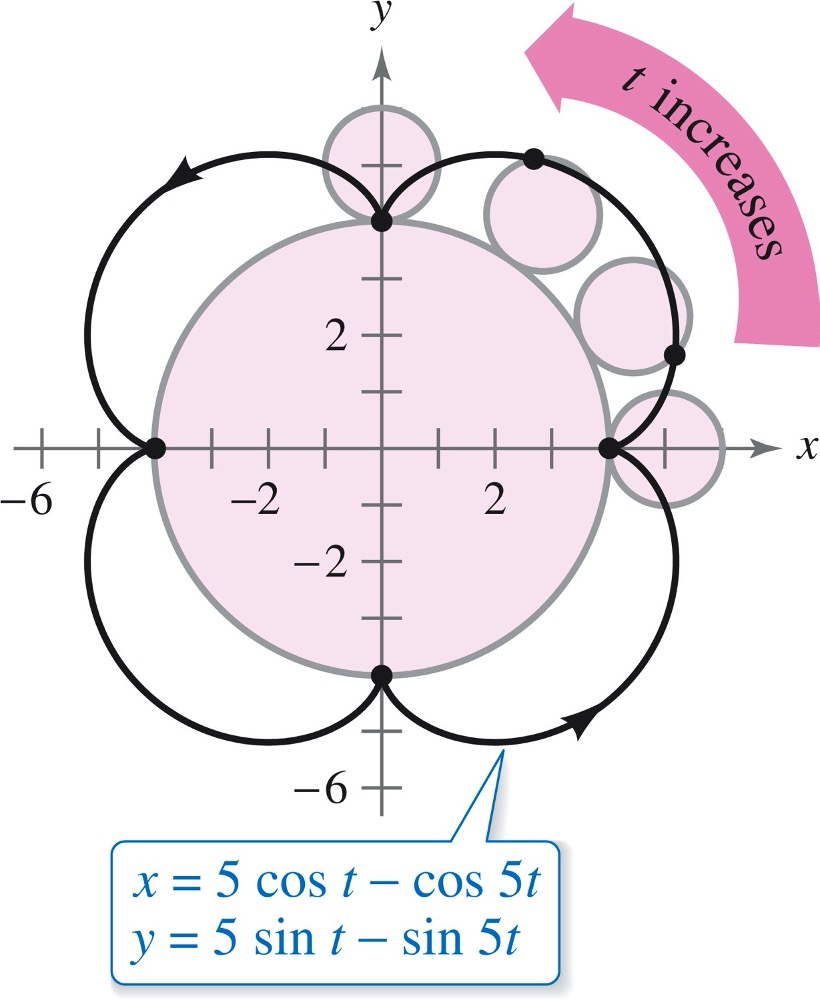
\includegraphics[scale=.2]{Picture3.jpg}
\end{center}

One complete trip around the larger circle occurs for
\[
0\leq t\leq2\pi.
\]
The epicycloid has four-fold rotational symmetry.  The portion of the curve
traced for
\[
0\leq t\leq\frac{\pi}{2}
\]
has the same length as each of the other three portions of the curve.
Therefore, we find the length of this portion and multiply by $4$.

We have
\[
\frac{dx}{dt}=-5\sin t+5\sin 5t
\]
and
\[
\frac{dy}{dt}=5\cos t-5\cos 5t.
\]
Therefore,
\begin{eqnarray*}
s
&=&
4\int_{0}^{\pi/2}
\sqrt{
\left(-5\sin t+5\sin 5t\right)^{2}
+
\left(5\cos t-5\cos 5t\right)^{2}
}\,dt\\
&=&
20\int_{0}^{\pi/2}
\sqrt{
(\sin 5t-\sin t)^{2}
+
(\cos t-\cos 5t)^{2}
}\,dt\\
&=&
20\int_{0}^{\pi/2}
\sqrt{2-2\cos 4t}\,dt\\
&=&
20\int_{0}^{\pi/2}
\sqrt{4\sin^{2}2t}\,dt.
\end{eqnarray*}
Since
\[
0\leq t\leq\frac{\pi}{2},
\]
we have
\[
0\leq2t\leq\pi,
\]
and hence $\sin 2t\geq0$.  Therefore,
\[
\sqrt{4\sin^{2}2t}=2\sin 2t.
\]
Thus,
\begin{eqnarray*}
s
&=&
40\int_{0}^{\pi/2}\sin 2t\,dt\\
&=&
40\left[-\frac{1}{2}\cos 2t\right]_{0}^{\pi/2}\\
&=&
40.
\end{eqnarray*}
Therefore, the point travels a distance of
\[
\boxed{40}.
\]

\end{enumerate}
\end{document}




















